\documentclass[12pt,a4paper,twoside,times,sky,standard]{csiroreport2017}

\usepackage{amsmath,amssymb,wasysym,bm}
\newcommand{\etal}{\textit{et al.}}
\newcommand{\ds}{\displaystyle}
\newcommand{\eps}{\epsilon}
\newcommand{\rp}{r^\prime}
\newcommand{\ap}{a^\prime}
\newcommand{\lp}{l^\prime}
\newcommand{\vphi}{\varphi}
\newcommand{\ty}{\tilde{y}}
\newcommand{\tl}{\tilde{l}}
\newcommand{\tr}{\tilde{r}}
\newcommand{\ttt}{\tilde{t}}
\newcommand{\ttmax}{\tilde{t}_{\rm max}}
\newcommand{\piret}{\pi^{\rm ret}}
\newcommand{\pirec}{\pi^{\rm rec}}
\newcommand{\pirep}{\pi^{\rm rep}}
\newcommand{\pp}{\mathbf{p}}
\newcommand{\uu}{\mathbf{u}}
\newcommand{\vv}{\mathbf{v}}
\newcommand{\tmax}{t_{\rm max}}
\newcommand{\tbz}{\tilde{\textbf{z}}}
\newcommand{\vtheta}{\vartheta}
\newcommand{\vphit}{\vphi^{\rm tag}}
\newcommand{\xtheta}{\mbox{\boldmath$\theta$}}


%Fill in the title, authors, in confidence text, etc as required.
%If you don't want one or the other then just comment them out.
%\docinconfidence[Commercial In Confidence]


\docdivision[Environment]


\docbusinessunit[
    CSIRO Environment\\
    Battery Point, Hobart 7000, Tasmania, Australia.\\
]


% The title of the document. Try to keep it to 3 lines or less.

\doctitle[\vspace{0mm}\huge Initial exploration of replacing the CCAMLR rule for Macquarie Island toothfish]

\docfootertitle[MITF initial MSE]

\docauthors[\vspace{4mm}\Large R. Hillary \& P. Bessell-Browne]

%\docreportnum[Report Number: CMIS 2009/00]

\docreportdate[26\textsuperscript{th} April 2024]

\doccopyrightyear[2024] % For the Copyright and Disclaimer notice


\begin{document}
%=================================================

\section{Background}

The Macquarie Island Patagonian toothfish fishery, as well as the majority of the CCAMLR-managed toothfish fisheries (HIMI, South Georgia, Ross Sea), are all managed via integrated stock assessments that are then used to generate an overall TAC via the CCAMLR Harvest Control Rule (HCR) - henceforth ``the CCAMLR rule''. The general working mechanism of the CCAMLR rule can be summarised as follows:

\begin{enumerate}
    \item Use current state of population from assessment to project forward
    \item Calculate (constant) catch where relative SSB above 50\% unfished with probability 0.5 after 35 years
    \item Calculate (constant) catch where relative SSB above 20\% unfished with probability 0.9 (all years)
    \item TAC is the \emph{lowest} of these two catches
\end{enumerate}

The initial context of the rule could be characterised as follows: given sporadic estimates of the abundance of a population, how can precautionary catch levels be set in place - possibly for an extended amount of time. Within the Australian fisheries context the CCAMLR rule as been applied consistently for over a decade for both the HIMI and Macquarie Island fisheries. The original context for the CCAMLR rule does not really apply to the current state of Australian toothfish fisheries. Both the major fisheries have mature, relatively complex integrated assessments that are capable of providing multi-decade reconstructions of both the population and fishery dynamics. They both have their advantages and challenges - and some of these layer onto the overall effectiveness of the CCAMLR management approach - but they have little in common with the original CCAMLR rule context. More importantly, the application of the rule has resulted in a number of negative performance behaviours:

\begin{itemize}
    \item TAC variability - there are no explicit constraints on the degree to which the TAC can vary from one decision to the next. Changes in excess of 20\% are quite common. This level of change is often hard-wired into other management procedures as a \emph{maximum} change and values well below this are considered good performance indicators
    \item Interaction with recent population dynamics - the constant catch, long-term projection nature of the CCAMLR rule has the tendency to amplify the effect of recent stock and fishery dynamics on the TAC
    \item Overall it is \emph{very} sensitive to the overall scale of the population coming from the stock assessment - at least in the last three TAC decisions at Macquarie Island this relationship has been almost a one-to-one relationship
\end{itemize}

The last point has further implications that are hard to quantify in relation to the TAC, but very impactful in relation to the management process. If the management advice is so strongly dependent on the stock assessment it becomes scientifically and practically very difficult to explore development and adaption of the assessment where the implications for the management advice are not influencing the process - both consciously and subconsciously. As important is the fact that the CCAMLR rule has never really been fully tested in the Management Strategy Evaluation (MSE) sense, where the full feedback dynamics of the whole system are simulated. 

The process of MSE is considered best practice when developing and evaluating fisheries management strategies \cite{mse}. Since its genesis in the International Whaling Commission \cite{iwc} it has shown repeatedly that two general observations hold true: (i) ``on paper'' good ideas for management strategies do not always work very well when tested against reality; and (ii) complex is not always better than simple in terms of ``assessment'' methods in management strategies - empirical or simpler model-based assessments often out-perform the current stock assessment model when tested concurrently. A schematic of the MSE process in a systems analysis sense can be seen in Figure 1.1

\begin{figure}[hb]
    \begin{center}
        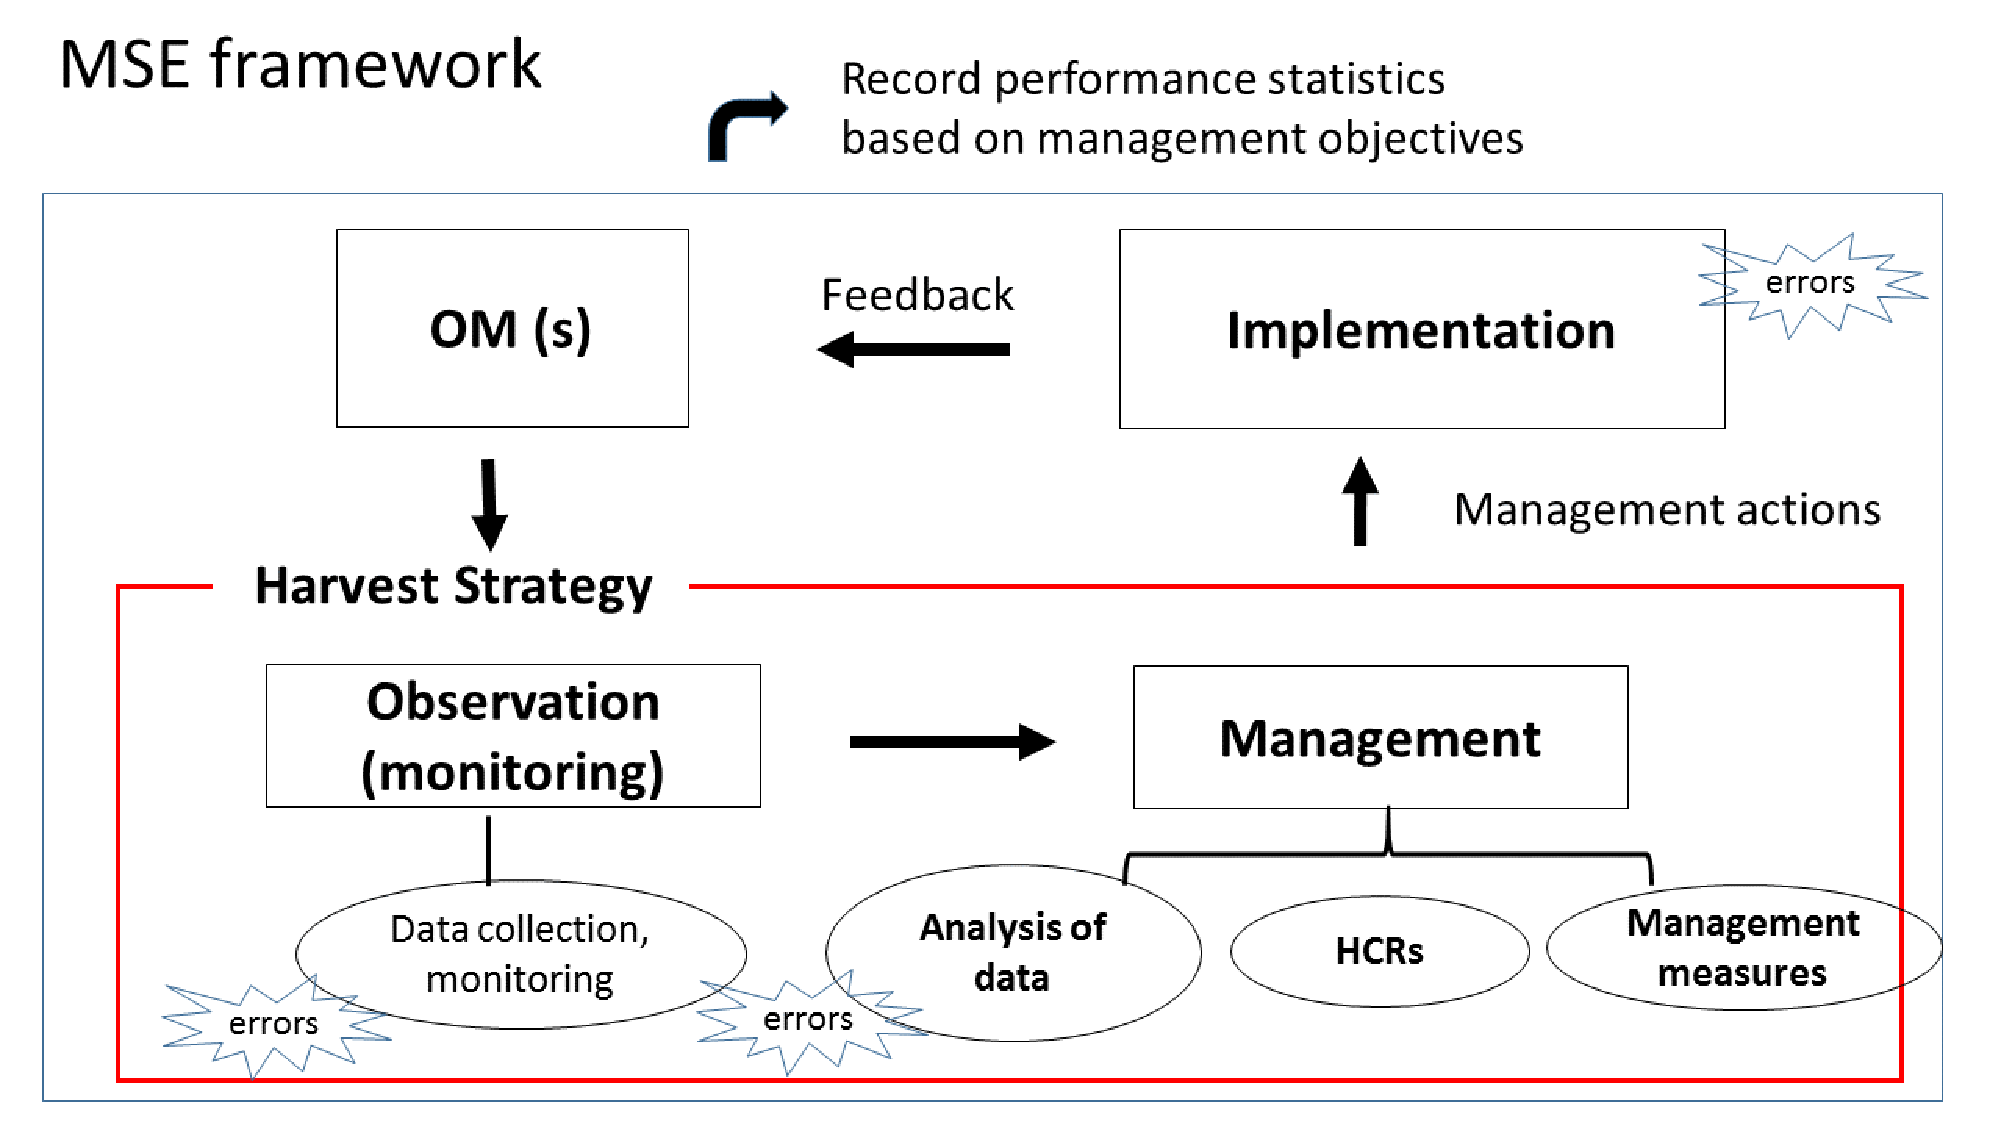
\includegraphics[width=11cm,height=7cm]{figs/MSE.pdf}
    \end{center}
    \caption{\textit{A system scale schematic of the MSE process. The red box encapsulates where the Management Procedure (harvest strategy) is embedded in the wider fishery system.}}
\end{figure}

This document is an initial exploration of what type of candidate Management Procedures (MPs) might be developed to replace the current CCAMLR approach (integrated stock assessment then use the CCAMLR rule). For Macquarie Island the major information source in relation to abundance and mortality is the tagging data, with additional key information from the age, length and maturity data. The stock assessment statistically integrates all these data sources to provide us with an estimated spatiotemporal reconstruction of the population and fishery dynamics for the resource \cite{misa}. Research from a large diversity of MSE examples and contexts \cite{mse,iwc,sbtmp,mprev} all give credence to the idea that either empirical or model-based MPs that are notably less complex than the stock assessment can not only perform well in managing a fishery, but can often perform \emph{better} than the stock assessment in this regard. In this initial tranche of MSE work we posit that the tagging data are the best candidate for a \emph{single} data set that could be used in a suite of candidate MPs. This does not suggest that there may not be additional beneficial information from the additional data (age and length composition) - this is clearly demonstrated in the stock assessment model \cite{misa}. However, the assessment also tells us that the dominant data set in relation to estimates of abundance and mortality is the mark-recapture data. So, while we do not rule out exploring the utility of including additional data as inputs to candidate MPs, the MPs proposed herein use \emph{only} the tagging data.

\section{Methods}

There are a number of general steps in a fully realised MSE loop:

\begin{itemize}
    \item Definition and conditioning of suite of Operating Models (OMs) that will generate population and fishery dynamics as well as the observations to be used in the candidate MPs
    \item Definition of the candidate MPs: (i) suite of input data; (ii) underlying ``assessment'' model; and (iii) HCR that uses assessment output and additional parameters to generate the relevant management action variable (e.g. TAC)
    \item A set of key management objectives for the candidate MPs to achieve and a suite of performance criteria against which we can assess relative performance across the candidate MPs
    \item A suite of past and/or future additional scenarios (a.k.a. robustness tests) to ascertain how robust the candidate MPs, which can acceptably achieve the key management objectives, are to alternate hypotheses about the state of the system under consideration  
\end{itemize}

\subsection{Operating Model structures}

Generally, OMs require \emph{at least} the nominal level of complexity of the stock assessment if one exists \cite{mse} but ideally they should have the capability of being able to model dynamics that are often far more complicated than the assessment. Features such as time/sex/size/age varying processes (e.g. growth, natural mortality, selectivity, migration) not modelled in the assessment are often included so as to be able to simulate the kind of features we want a candidate MP to be robust to. The OM needs to (i) simulate the population and fishery dynamics in response to population (endogenous) and environmental (exogenous) factors, and the exploitation of the resource by the fishery; and (ii) simulate the suite of observations we intend to use in the candidate MPs.

The population dynamics in the OMs we employ are year/age/length/sex/spatial in general structure, as is the stock assessment \cite{misa}, with the additional capability to permit temporal structure in various population (recruitment, natural mortality, growth) and fishery (selectivity, fishing location) processes. It can also accommodate sex/age/size structure in processes such as natural mortality and migration if required. For the data simulation part of the OM we need to define a suitable suite of observation error models. These connect the population and fishery dynamics to an appropriate generating probability distribution. Within the MSE software suite we can generate:

\begin{itemize}
    \item Mark-recapture data: focus is on tag release covariate conditional estimators (the Brownie suite of models) so this is how they are simulated (with over-dispersion included) in the observation error model
    \item Length data: length composition by fishery via the Dirichlet-multinomial
    \item Age-given-length data: by fishery via the multinomial distribution
    \item Relative abundance indices: surveys, fleet-specific CPUE indices via either the multivariate or simpler log-normal distribution
\end{itemize}

For the simulation of the tag data the probabilities we model the tag release dynamics of each release ``event'' i.e. all the releases in a given year, sex, age class and spatial region. The probability of recapturing a tag depends on tag shedding and mortality, natural mortality, the harvest rate, and the spatial transition matrix. Though the underlying generating distribution is assumed to be a Dirichlet-multinomial we use the conditional beta-binomial generating method. This is because as we move forward in time we are releasing tags in a given release ``cohort'', recapturing them, using the data in a TAC decision year but also recapturing the same releases further ahead in time. So we cannot simply use the Dirichlet-multinomial distribution to simulate the data - instead we use the beta-binomial distribution to simulate recaptures in the given time period, and as we project forward in time we use the conditional sampling approach to simulate future recaptures in the same release group. This preserves both the marginal distributions of each possible recapture event, as well as the implicit negative correlation in the multinomial (more/less recaptures ``early'' means less/more recaptures probable ``later''). The tag release age distribution is statistically inferred from the actual size distribution of animals at Macquarie Island (in this case) using the length-at-age distribution (by sex), and the number of releases is dictated by an assumed tag-per-tonne release rate, the catches by region, and the estimated sex and age distribution of releases.

\subsection{Mark-recapture estimators}

There are several main groups of tag estimators (and variations within each) but for Macquarie Island toothfish the two main groupings have been the modified Petersen (Stock Synthesis) and the Brownie - the spatial sex and length structured Brownie is used the current assessment \cite{revass2019}. The reason for moving to the spatial Brownie approach to modelling the tagging data was driven by the side-by-side comparison of the Stock Synthesis approach (two-stage negative binomial and spatial multinomial) and spatial Brownie focussed on the relative accuracy of their estimates of both spawning abundance and migration rates \cite{tagdes}.

The Brownie estimator is release conditional and it models the future recapture of tagged animals only within a given release event - it doesn't model pooled tag releases and recaptures as some Petersen-style estimators. The probability of recapturing a released tag is constructed via a two-stage process:

\begin{enumerate}
    \item Calculate the probability that a tagged fish survives the tag release process, still has \emph{at least} one tag still attached, survives both natural mortality and fishing \emph{and} is located in the spatial region of interest
    \item Conditional on the first probability, calculate the probability that the tag is recaptured \emph{and} reported
\end{enumerate}

For the spatial Brownie estimators we propose to use for the candidate MPs the structure is simplified by removing the dependence on either age (length) or sex of release as is done in the stock assessment. Additionally we also explore non-spatial estimators even if there is underlying spatial structure in the population dynamics and underlying mark-recapture data. By simplifying in this way (removing the dependence on age/length/sex at release) what these estimators are estimating will be close to what the average harvest rates would be coming from the stock assessment. The mathematical and statistical details of the suite of mark-recapture estimators can be found in the Appendix. It is not essential to obtain unbiased estimates of the true harvest rates - what matters is that there is a close correlation between the true harvest rates and those coming from the mark-recapture estimators. The process of tuning key HCR parameters can deal with any average bias and so if the estimates correlate well with the true values then any candidate MP should have useful estimates of the true harvest rate(s). All the mark-recapture estimators were coded in Template Model Builder \texttt{TMB} \cite{tmb} - the \texttt{R} package used to code the integrated stock assessment.

\subsection{Candidate Management Procedures}

There are two main derived quantities coming from the mark-recapture estimators and other fishery data:

\begin{enumerate}
    \item Harvest rates: overall/spatially averaged, $h_y$, or spatially explicit, $h_{y,r}$
    \item Exploitable abundance/biomass: given catch numbers/biomass, $C_y$, the exploitable abundance/biomass can simply be calculated by $X_y=C_y/h_y$ or $X_{y,r}=C_{y,r}/h_{y,r}$ in the spatial case and $X_y=\sum_r X_{y,r}$
\end{enumerate}

In very general terms these two variables present where the stock is ``going'' (harvest rates) and where the stock is ``at'' (exploitable abundance). In practice we could use both of these variables or just one in a candidate MP - for example the ``classic'' $\{F,SSB\}$ hockey-stick HCR used in for example the SESSF, EU and elsewhere can be mirrored to a degree using an analogous $\{h,X\}$ HCR. In practice, there are several reasons why these types of rules don't always perform as well as other often simpler approaches, but one can explore what might be termed familiar types of HCR using the estimates from the mark-recapture models.

In this initial work we explored a relatively straightforward general framework for the HCR in a given management decision year, $y$:

\begin{equation*}
    \ds TAC_{y+1}=TAC_y\times\Delta_y
\end{equation*}
where the TAC change is defined by
\begin{equation*}
    \ds \Delta_y=\min\{1+\delta_{\rm max},f(h,X,\xtheta)\}
\end{equation*}
if $\Delta_y>1$ and 
\begin{equation*}
    \ds \Delta_y=\max\{1-\delta_{\rm max},f(h,X,\xtheta)\}
\end{equation*}
if $\Delta_y<1$ and $f(h,X,\xtheta)$ is the HCR response function (with HCR parameters $\xtheta$) but the TAC change in a given decision year is bounded by $1\pm\delta_{\rm max}$. The built-in feature of this type of overall HCR an innate level of TAC stability and consistency given the next TAC is always constrained to be some maximum distance from the current one. 

One of the simplest HCRs we can construct is a target-based HCR based on the recent mean harvest rate. Define a recent moving average harvest rate as follows:
\begin{equation*}
    \ds \bar{h}=\sum\limits_{i=y-\tau+1}^y h_y,
\end{equation*}
where $\tau$ is the length of time over which the moving average is taken. Also define a ``target'' harvest rate $h^{\rm targ}$, then our HCR response function can be defined as
\begin{equation*}
    \ds f(h,\xtheta)=\left(\frac{h^{\rm targ}}{\bar{h}}\right)^\nu
\end{equation*}
so $\xtheta=\{h^{\rm targ},\nu,\tau\}$ and $\nu$ is a response parameter such that for $\nu>1$ the HCR is superlinear and for $\nu<1$ it is sublinear in its response. Initially we simply explore $\nu=1$ but there are often cases where we want to dial up (or down) the responsiveness of the HCR and this kind of parameter is a straightforward and interpretable way to do this. This type of HCR will increase/decrease the TAC if the recent mean harvest rates are below/above the target. The main tuning parameter in this HCR would be the target harvest rate, $h^{\rm targ}$ - to be clear this is just a parameter of the HCR, not a feature of the true dynamics of the OM. Even if we set the main objective to be attaining $SSB_{\rm msy}$ and tuned this MP to achieve that objective it does not mean that $h^{\rm targ}\equiv h_{\rm msy}$. Parameters of any HCR are useful degrees of freedom that can be altered or tuned directly to achieve a given set of objectives or performance characteristics and do not need to have interpretable counterparts in concepts like MSY or MEY for example, even if they are tuned to achieve those objectives. 

\subsection{Management objectives \& performance statistics}

Even in data poor settings, it is important to clearly specify a single objective (or set of multiple objectives) for candidate MPs to achieve as a base level of performance \cite{mse}. Once those objectives are set we then need a suite of performance statistics against which we can ascertain relative performance across candidate MPs. Ideally both these processes - setting objectives and deciding performance measures - should be guided by practitioners but driven strongly by policy makers and stakeholders. To obtain stakeholder buy-in and commitment to an MP it should be these groups that decide what they want an MP to achieve, and what kinds of behaviours they would like to see in the candidate MPs in \emph{how} they achieve the objectives. 

For this initial work we explored a simple management objective that the candidate MPs had to be tuned to: attain a (female) spawning stock biomass of 50\% of the unfished level with probability 0.5 at some pre-defined year (or set of years) in the future after the implementation of the MP. In terms of performance statistics there are obviously many that could be envisage but some very common ones are:

\begin{itemize}
  \item Probability that the (female) SSB falls below a given limit reference point (LRP) if one exists
  \item Average TACs for different future time periods
  \item Average annual variation (AAV) in TAC - often expressed as a percentage and the mean percentage change in TAC when a management decision is made
  \item The potential trade-off between average TAC and AAV - often they are negatively correlated (more flexible MPS can attain higher TACs but do so at the cost of more variability in TAC)
  \item Proportion of times a TAC decision triggers the maximum change condition - if this is high our MP is approximating a discrete switch function and is probably too responsive to the inputs
  \item Some kind of fishery efficiency performance statistics such as CPUE or inferred effort - or even profitability measures if some basic economic data are available
\end{itemize}

There are obviously many more that can be explored and the general rule is this: if we simulate it we can summarise it, but don't create too crowded a performance picture as it can be hard to make inferences with too many statistics.

\subsection{Robustness tests}

The general process of tuning an MP \cite{mse,sbtmp} is twofold:

\begin{enumerate}
    \item To ensure that - at least - all candidate MPs can achieve the state management objectives
    \item To ensure a level playing field between candidate MPs so that one can better assess their performance characteristics given they all have to achieve a specific management objective
\end{enumerate}

Once we have tuned a suite of candidate MPs, and inspected the performance statistics to assess any performance differences between them, the next stage in the MSE process is to see how robust they are to alternate hypotheses about the stock dynamics. Generally, the most likely suite of parameter and process hypotheses is included in the reference set of OMs used to tune the candidate MPs \cite{mse,sbtmp}. The robustness tests tend to include less likely scenarios - less supported by the data, for historic processes, or future scenarios that have not yet been seen but are considered plausible or important.

Somewhat naturally these tests separate into fishery and population dynamic groupings. In the Southern bluefin tuna example \cite{sbtmp} fishery robustness tests focussed on alternative hypotheses about past and future longline catchability (CPUE index is used in the MP) and the relationship between abundance and CPUE. Population dynamic scenarios related to future recruitment failure (given a previous prolonged period of low recruitment in the recent past) and alternative abundance indices that resulted in different stock status outcomes in the historical dynamics. 

For the Macquarie Island case there are not too many obvious fishery related robustness tests beyond fishing location dynamics (relative to the North/South divide). There is a single boat and we do not use effort directly or CPUE as an abundance index so no catchability issues to explore beyond perhaps in performance statistics. In terms of population dynamics there are some focal points: (i) size/age structured migration and changes over time given we have a spatial model; (ii) future changes in growth given observed shifts in weight-at-length in relation to possible environmental changes; (iii) future changes in recruitment dynamics (spatial split, regime changes in the average level). The MSE process is a more natural place to deal with the issue of climate change and sustainability because environmental effects are hard to include directly in the stock assessment process, and often really involve future scenarios relating to the population dynamics.

\subsection{Simple example}

To demonstrate the MSE process we employed a Macquarie Island toothfish like example case study:

\begin{itemize}
    \item Essentially the same life-history parameters (growth, maturity, natural mortality), fishery characteristics (long-line, selectivity parameters), and spatial set up (two areas with 10\% annual movement for all ages)
    \item The population begins at the unfished state with a fixed harvest rate fishing strategy for 20 years before the MP is implemented. The fixed harvest rate is the value that will attain a female SSB depletion level of 0.5 at deterministic equilibrium
    \item Ten years after fishing commenced an annual tagging program at 3 tags-per-tonne is initiated 
    \item After twenty years of fishing when the tagging data has sufficiently accumulated we assume an MP is implemented with a TAC decision made every 5 years
    \item The projection goes for 20 years and the candidate MPs are tuned achieve a female SSB level of 50\% of unfished with probability 0.5 in the final year of the projections (i.e. 20 years after MP implementation)
\end{itemize}

This is a simple almost exploratory fisheries scenario but it is a useful  in that it can outline several key features of relevance to the Macquarie Island fishery. In terms of candidate MPs we explored two:

\begin{enumerate}
    \item \textbf{MP1}: uses spatially/sex/age aggregated tagging data using the non-spatial mark-recapture estimator and estimates the random effect variance of the harvest rate year effects. The fixed HCR parameters are $\tau=4$ and $\nu=1$ with $h^{\rm targ}$ the tuning parameter
    \item \textbf{MP2}: uses sex/age aggregated but spatially structured tagging data using the spatial mark-recpature estimator (estimating area-specific harvest rates and migration parameters jointly)  with the random effect variance of the harvest rate year effects estimated also. To get an overall harvest rate the MP uses an average of the region-specific harvest rates (weighted by the relative catch split). The fixed HCR parameters are $\tau=4$ and $\nu=1$ with $h^{\rm targ}$ the tuning parameter
\end{enumerate}

\section{Results}

As well as summarising the initial example MSE scenario in this section we also outline how well the two main non-spatial and spatial mark-recapture estimators perform on the actual Macquarie Island toothfish fishery tagging data. This is to demonstrate that these simplified estimators can go along way to replicating the key features of the estimates of harvest rates (and migration in the spatial case) coming from the stock assessment. 

\subsection{Example MSE results}

Both \textbf{MP1} \& \textbf{MP2} were tuned (via the $h^{\rm targ}$ HCR parameter) to meet the example management objectives. We summarised their performance using five main statistics:

\begin{enumerate}
    \item Relative (female) SSB in the middle of the projection period (10 years from the implementation of the candidate MPs)
    \item Relative (female) SSB at the end of the projection period (20 years from the implementation of the candidate MPs)
    \item Time-averaged TAC for the projection period after MP implementation
    \item The AAV in the projection period when the MP is active
    \item The probability that the maximum TAC change constraint is triggered in the active MP projection period
\end{enumerate}

Figure 3.1 summarises the performance statistics we calculated for the two candidate MPs. Clearly the performance of the two candidate MPs is very similar. They are both tuned, within a tolerance of 1\%, to obtain the same final relative SSB and we see a very similar distribution around the tuned median depletion at the end of the projection period. In terms of average TACs the medians are very similar - a little higher for \textbf{MP2} but also a little more variable - as are the AAV statistics, though for \textbf{MP2} the distribution is a little narrower. The probability that the maximum TAC change constraint was triggered for \textbf{MP1} and \textbf{MP2} was and 0.015 and 0.011, respectively.

\begin{figure}[hb]
    \begin{center}
        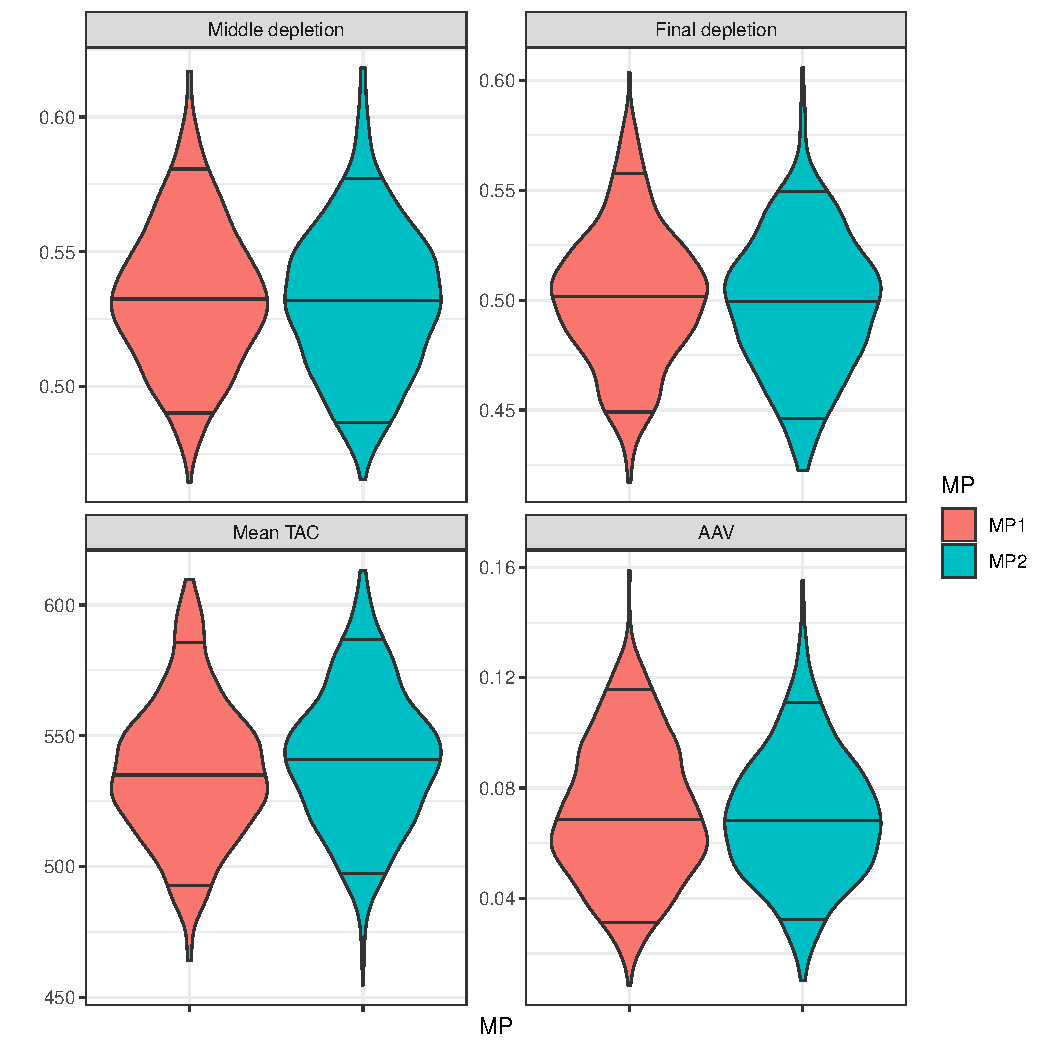
\includegraphics[width=11cm,height=10cm]{figs/fixedh_mpcomp.pdf}
    \end{center}
    \caption{\textit{Performance summary of the two tuned candidate MPs. The quantiles within the violins are the median and approximate 90\%iles.}}
\end{figure}

Figure 3.2 graphically summarises the time evolution of the key population and fishery dynamics: relative female SSB, TAC and average harvest rates. We only show them for \textbf{MP1} given they are very similar for \textbf{MP2}. In the 20 year initial period the effort (harvest rate) is kept constant at the equilibrium value that would result in a (deterministic) SSB depletion of 0.5, and we see the spawning population gradually declining towards this level but is still above it (median value of around 0.61) by year 20. The candidate MPs are tuned to attain an SSB depletion of 0.5 (with probability 0.5) by year 40, which would not happen in the fixed harvest rate initial scenario it would take longer. As a result, the candidate MPs initial increase the harvest rate (and TACs) to achieve this objective. By the third and fourth TAC decision the candidate MPs begin to then decrease the catches (and harvest rates) as the spawner biomass declines towards the target.

\begin{figure}[hb]
    \begin{center}
        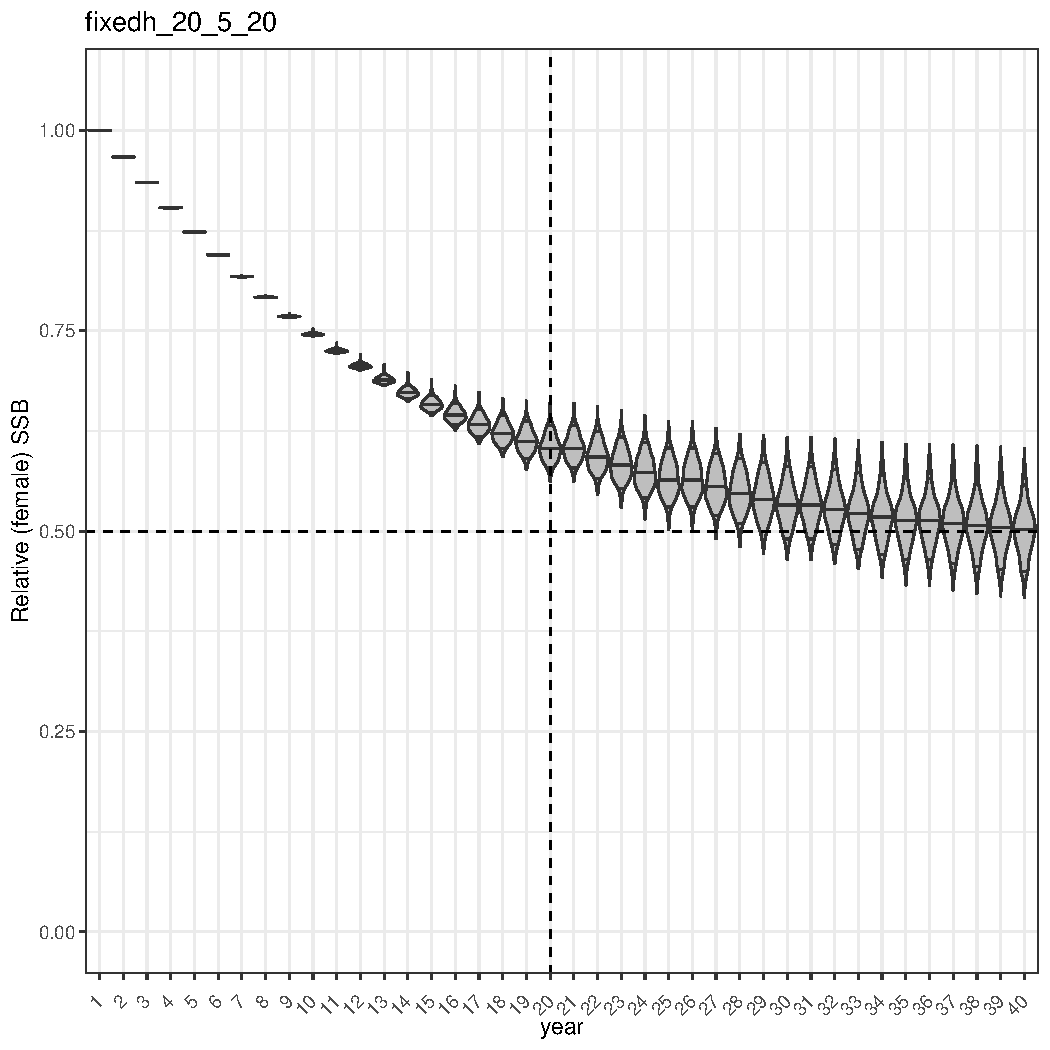
\includegraphics[width=5cm,height=5cm]{figs/fixedh_dep.pdf}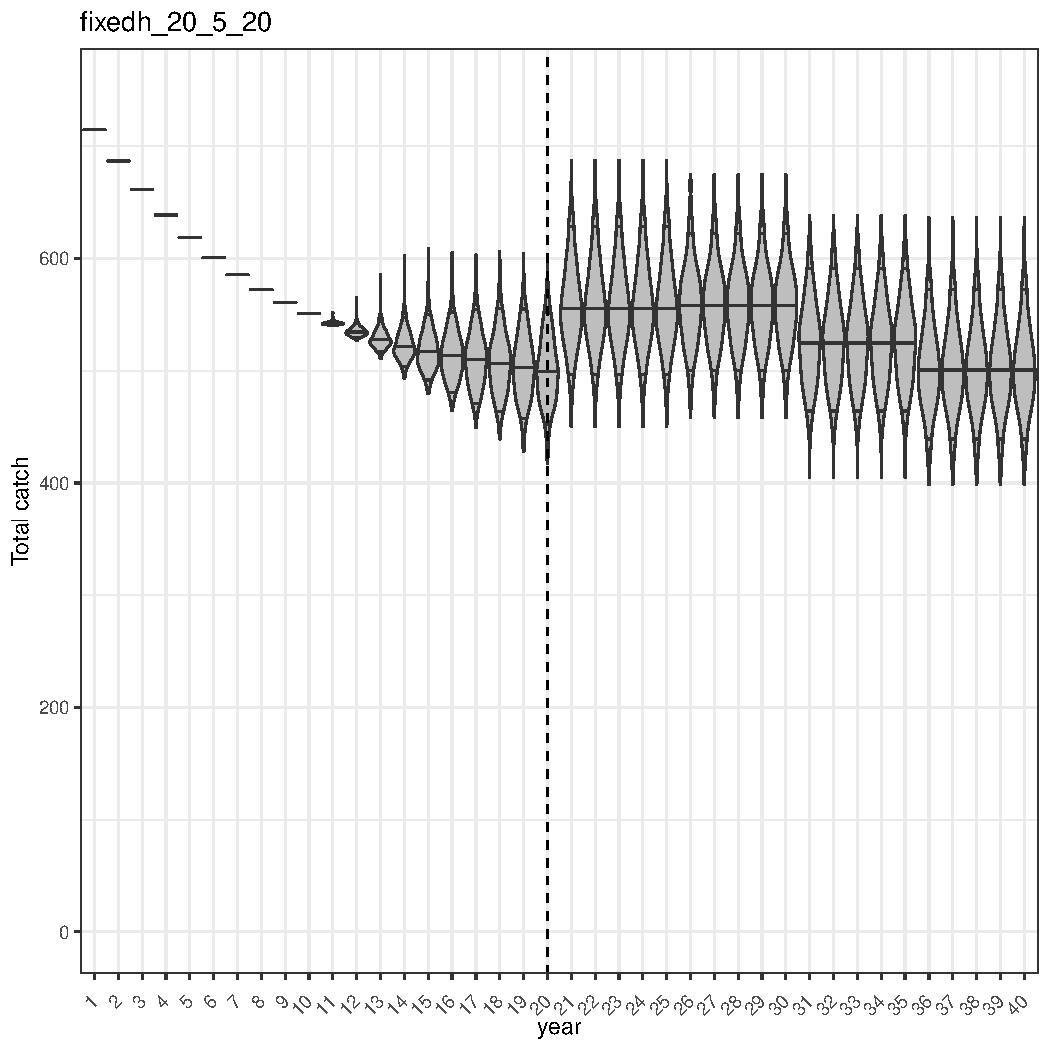
\includegraphics[width=5cm,height=5cm]{figs/fixedh_tac.pdf}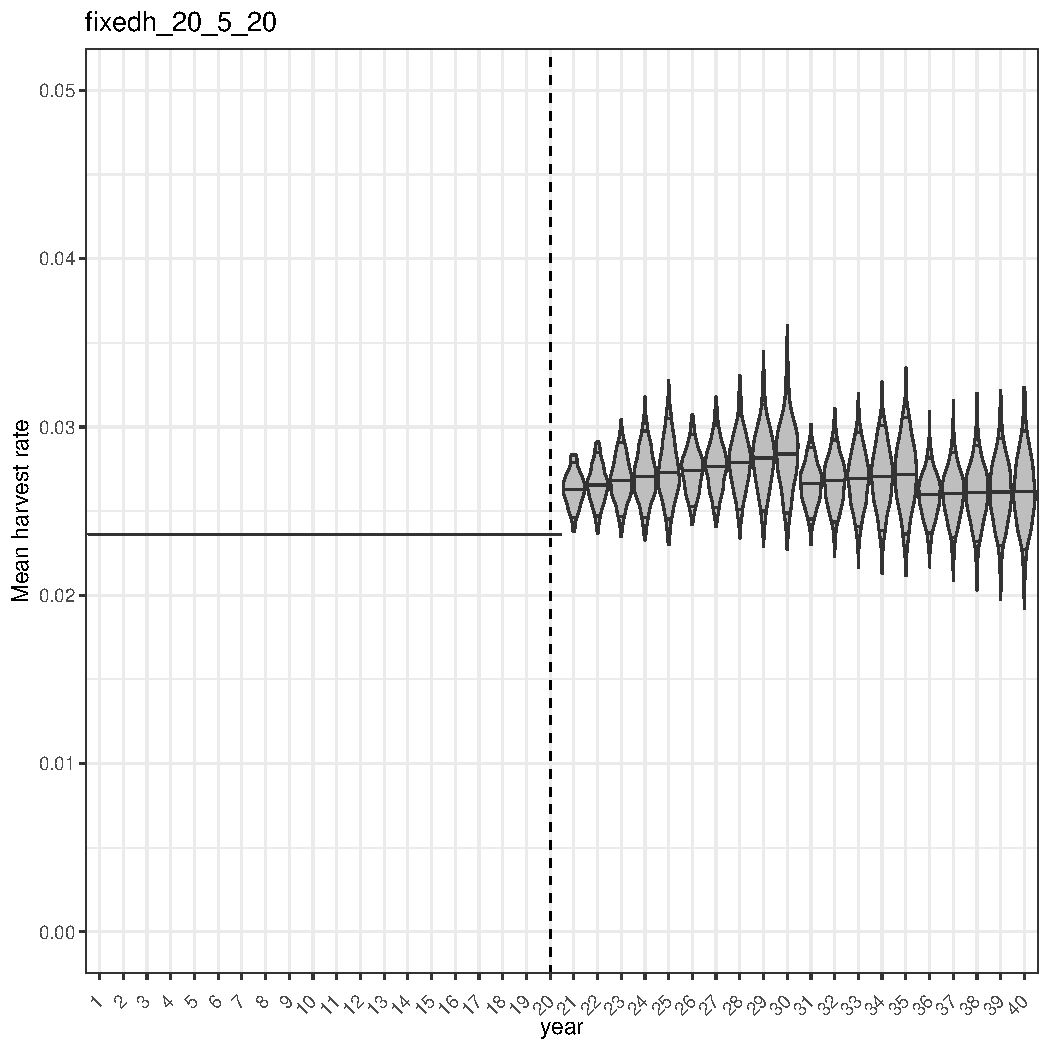
\includegraphics[width=5cm,height=5cm]{figs/fixedh_hrate.pdf}
    \end{center}
    \caption{\textit{Time evolution summary of the relative female SSB (left), TAC (middle), and the average harvest rate (right). The quantiles within the violins are the median and approximate 90\%iles.}}
\end{figure}

\subsection{Tagging estimators and Macquarie Island tagging data}

An informative test of any model-based candidate MP is: how well does to explain the actual observed data? The general form of the mark-recapture model proposed in this paper (spatial and non-spatial Brownie models) is very similar to the more complex form in the stock assessment, where length, sex and region of release are the key covariates that dictate data aggregation level. We fitted the spatial and non-spatial versions of the suggested MP estimators to the actual Macquarie Island tagging data used in the 2021 assessment. The non-spatial model estimates year-specific harvest rates (in terms of a mean and annual random effect parameter) and the variance of those annual random effects. The spatial model estimates year-specific harvest rates (mean and RE deviation) for each region as well as the migration probabilities between the two North and South regions as defined in the stock assessment. 

\begin{figure}[hb]
    \begin{center}
        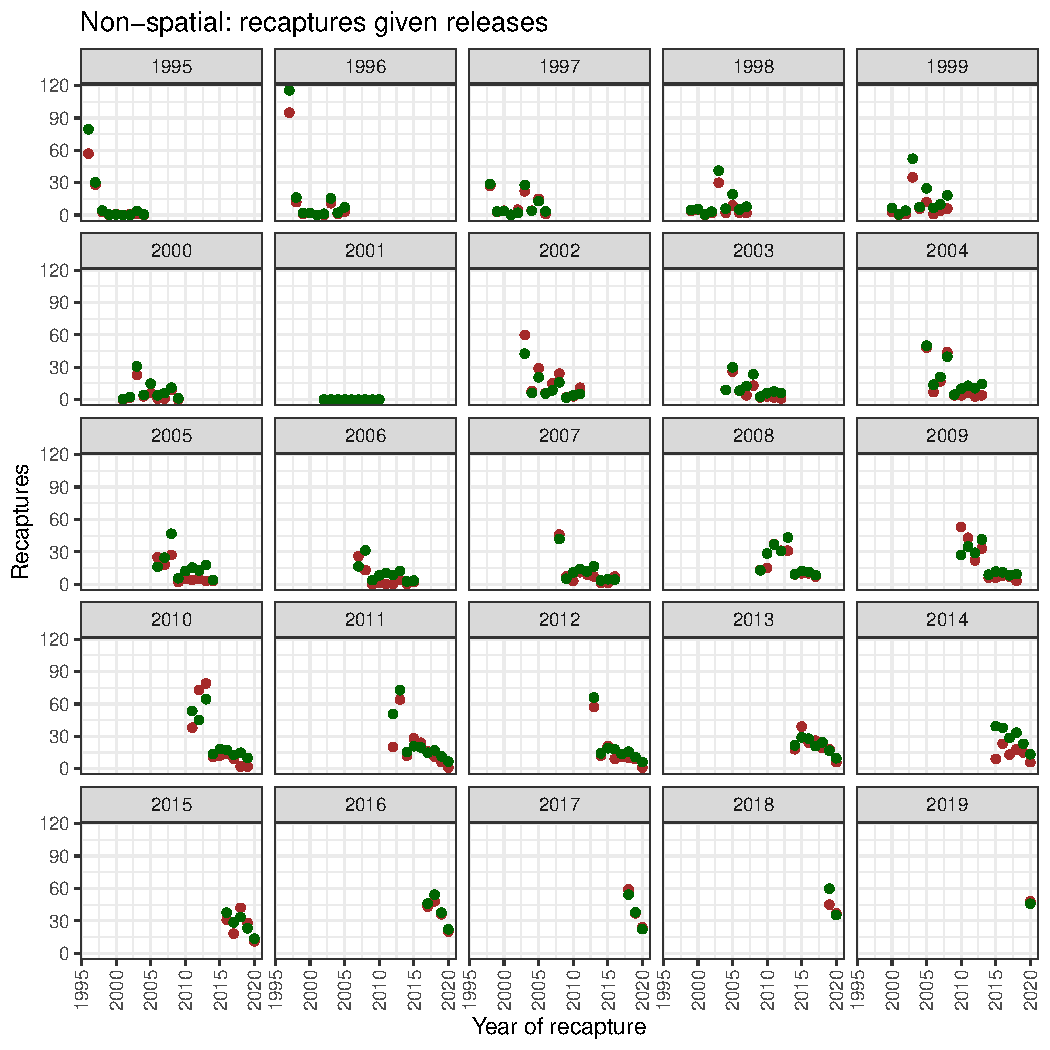
\includegraphics[width=6cm,height=6cm]{figs/nonspfits_macca.pdf}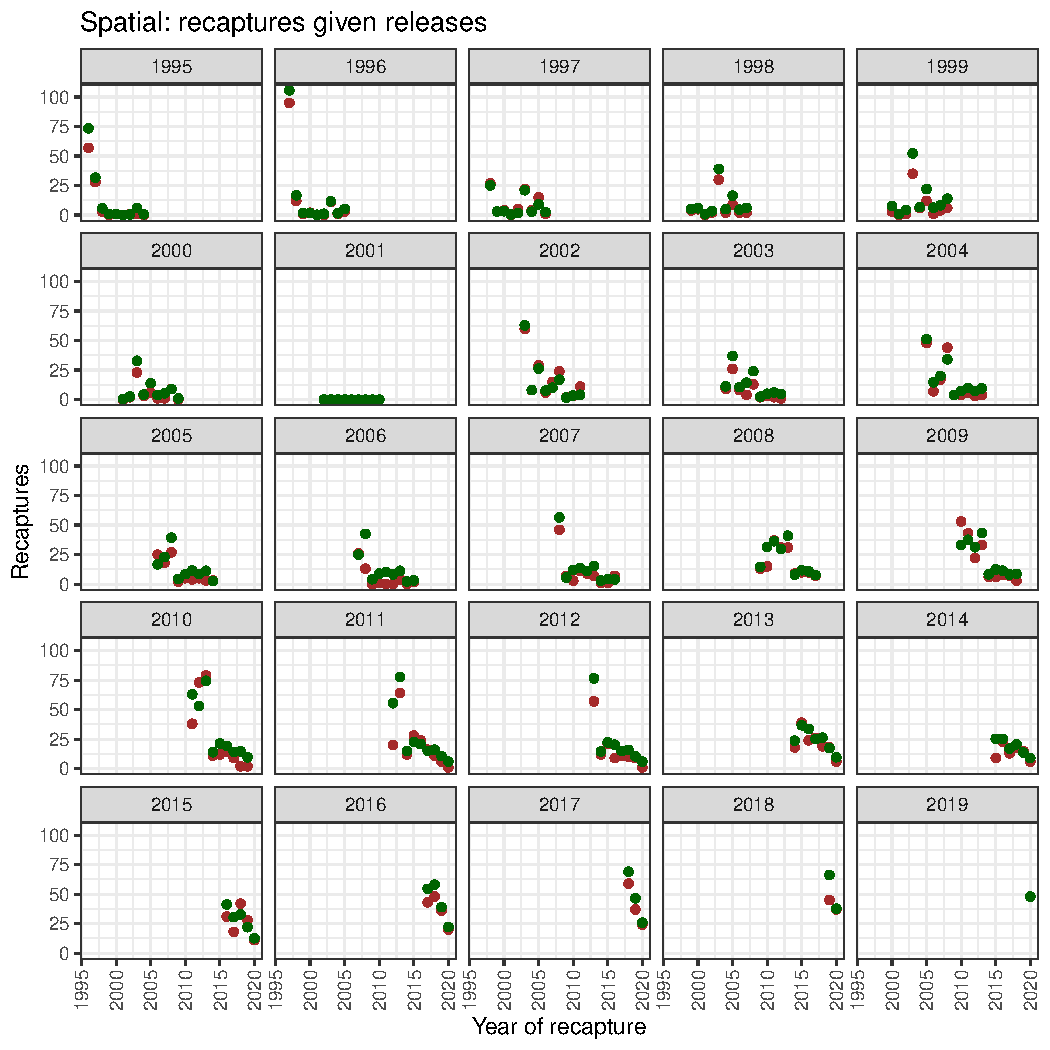
\includegraphics[width=6cm,height=6cm]{figs/spfits_macca.pdf}
    \end{center}
    \caption{\textit{Fits to the Macquarie island tagging data (from the 2021 assessment) for the non-spatial (left) and spatial (right) models. The brown dots are the observed data and the green are the predictions. Each panel corresponds to a release year and displayed are all the recaptures in the years following release.}}
\end{figure}

Figure 3.3 compares the spatially aggregated fits to the Macquarie Island tagging data for both the spatial and non-spatial estimators. Both models tend to explain the data reasonably well. Basically, they explain the data as well - in this spatially/sex/length aggregated summary - as the stock assessment \cite{misa}. It can be hard to see clearly from the visual summary in Figure 3.3 but the spatial estimator performs better (in the statistical significance sense of the word) than the non-spatial estimator. Figure 3.4 summarises the spatial disaggregated fitting summary when using the spatial estimator. 

\begin{figure}[hb]
    \begin{center}
        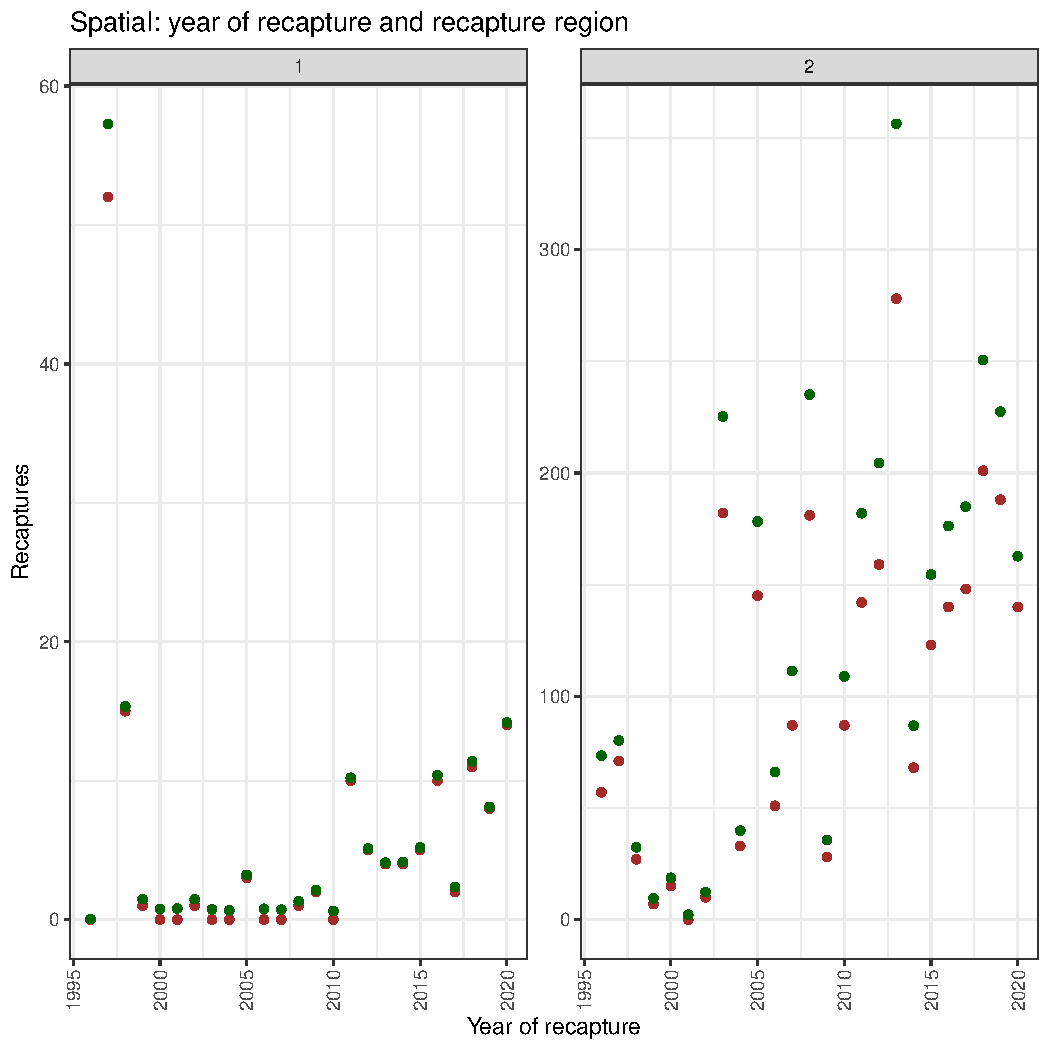
\includegraphics[width=9cm,height=7cm]{figs/spfits_recyrreg_macca.pdf}
    \end{center}
    \caption{\textit{Fits to the Macquarie island tagging data (from the 2021 assessment) for the spatial models. The brown dots are the observed data and the green are the predictions. Each panel corresponds to a recapture region and displayed are all the recaptures in that region in those years.}}
\end{figure}

In terms of harvest rate estimates Figure 3.5 summarises the spatial estimator's harvest rates for each region with the mean (averaged across sex and age) estimates coming from the 2021 stock assessment. Clearly in the early trawl period the simpler spatial estimator over-estimates harvest rates especially in the earliest period (1994--1998). However, as we move into the long-line regime (from around 2009 onwards) the estimates are far closer together. The reasons for this are twofold and interacting:

\begin{enumerate}
    \item The tag relese distribution is \emph{generally} on smaller fish that seen across the long-line distribution, and more in-line with the smaller fish caught in the trawl. This increases the probability of recapture (per unit of catch) in the trawl relative to the longline yielding higher recapture rates even for lower harvest rates driven by this differential availability in the two fisheries
    \item Recruitment deviations are more influential on recaptures in the trawl fishery relative to the longline for the reasons outlined above and a short period of notably weaker year-classes in the late 1980s/early 1990s in the assessment further increased the recapture probability of tags in the trawl fleet in the early tag repcature period
\end{enumerate}

Firstly, the points above suggest these types of estimators are going to potentially perform better, in terms of capturing average harvest rates, for the longline recaptures. Secondly, in the later longline dominant period the simpler estimators seem to capture mean harvest rates fairly well by area - this is precisely the input we are proposing to use in the candidate MPs outlined herein. In terms of movement estimates the N-to-S movement probability was 0.01, and the S-to-N estimate was 0.03 - the same as the 2021 assessment for N-to-S and under-estimated for S-to-N which was around 0.08. Again, the effect of selectivity - not accounted for in the simpler estimators - is the main driver for under-estimating movement. In the true tag dynamics the releases are mostly still in the ascending limb of the longline selectivity and, as such, are that much less likely to be recaptured even if they did move from S-to-N. In the simpler estimators we have no selectivity effect so the model interprets this as lower estimates of movement. 

\begin{figure}[hb]
    \begin{center}
        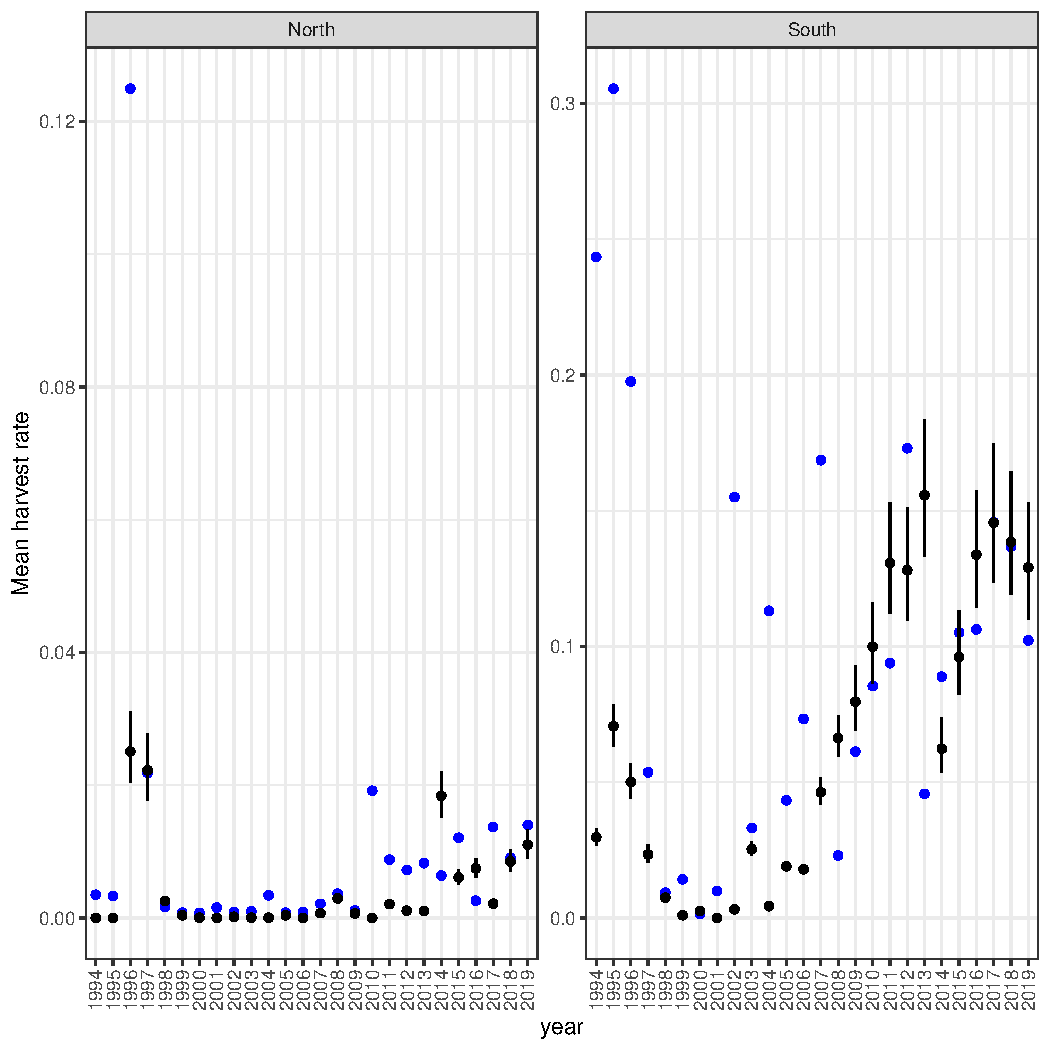
\includegraphics[width=9cm,height=7cm]{figs/hbarcomp_mpvstkass.pdf}
    \end{center}
    \caption{\textit{Estimates of mean harvest rates by region (the two panels) from the stock assessment (black in terms of median and 95\% credible intervals) and for the simple spatial estimator (blue points).}}
\end{figure}

\section{Discussion}

For both the Macquarie Island and HIMI Patagonian toothfish fisheries there  has been a number of years of discussion about what might replace the CCAMLR rule as the primary management advice instrument. It has been considered best practice to use the MSE process to develop and test alternative management strategies for a number of years \cite{mse} and in this paper we performed some initial exploratory work to develop and test candidate Management Procedures using the tagging data given this is the major data source for Macquarie Island. In this work we do not use the complex integrated stock assessment as the data analysis method; we use a simplified suite of mark-recapture estimators to obtain harvest rate estimates to use in the Harvest Control Rules. We could, in principle, use the full stock assessment as the analysis method but there are several reasons why we either don't need to or might not want to:

\begin{enumerate}
    \item Complexity: when testing methods from simple empirical MPs all the way to integrated stock assessment models the most complicated model doesn't always perform best. In fact, there often appears to be a range of complexity between the simplest empirical rules and the assessment that yields as good as if not better performance \cite{mse,iwc,sbtmp,mprev}. Additionally, with complicated assessments, such as those for toothfish \textit{spp.}, understanding and explaining how new data and model changes affect outcomes can be very hard to do definitively. Simpler analysis methods are far more amenable to stakeholder understanding of why an MP makes a given decision
    \item Testability: stock assessments are not fixed points, and each time they are run they often require human decisions on any changes required. These are effectively impossible to include in the MSE testing process, so if we test a single fixed version of the assessment in the MSE loop we are not truly testing the process of management via the outcomes of the stock assessment
    \item ``Separation of powers'': decoupling the assessment from the setting of management advice is a widely accepted additional benefit of the MP approach \cite{iwc,sbtmp}. Obviously, when the assessment effectively sets the management advice there is both conscious and unconscious pressure on decision making. This can inhibit the ability of analysts to develop the assessment over time, as well as the ability of a given working group to make either required or impactful decisions (so-called ``decision paralysis'' \cite{sbtmp})
\end{enumerate}

To develop the Operating Models required for the MSE testing process we generalised the underlying population and fishery models used in the stock assessment \cite{misa}. We have sex/age/spatial/size structured dynamics as well as the ability to explore a number of stage (age/sex) or time varying processes for growth, natural mortality, migration, selectivity and recruitment. Given we do not use effort or CPUE in the assessment there is less of a focus on fleet dynamic capability besides the choice of where to fish in a given season. We are able to generate statistically well-defined observations such as (spatiotemporal) mark-recapture data, length/age composition, age-given-length data, and survey abundance indices. The models are custom written in the \texttt{R} statistical language and are highly extendable in relation to alternative hypotheses about the relevant processes - both historical and in the future.

Given this is the first major piece of fully realised MSE work the SARAG has seen in relation to alternatives to the CCAMLR rule, we have included only a Macquarie Island-like simple example. The aim of the work was to set the scene for how we propose to develop new management approaches. The project currently envisages a two-step/two-year process whereby the initial work will be presented and discussed at this meeting of the SARAG. Based on feedback and suggestions at this meeting we would then develop a suite of suitable OMs and candidate MPs for the actual Macquarie Island fishery and report back to the first SARAG meeting in 2025.

For the simple Macquarie-like MSE example the OM began the population in unexploited equilibrium, with 20 years of fishing at the fixed effort (harvest rate) level that would eventually reduce the population to 50\% of the unfished level. After the first ten years of fishing tags were released into the two spatial regions. After the initial 20 years candidate MPs were then implemented that use the tagging data and make a TAC decision every 5 years with 20 years of projections into the future. Each of the two candidate MPs (one spatially explicitly, one using spatially aggregated tagging data) used a relatively simple target harvest rate HCR and were tuned (using the target parameter) to achieve a median relative (female) SSB of 50\% of the unfished level by the final year. The only additional constraint in the candidate MPs was that the maximum percentage change in TAC - up or down - was 20\%.

To assess relative performance of the two tuned candidate MPs we calculated several performance statistics: ``mid-way'' and final relative SSB, average catch over the projection period, and average variation in TAC when a management decision is made. Both candidate MPs performed very similarly, which was not surprising given the even population spatial distribution and relatively low level of migration between the two regions (10\%). The MP with the spatial mark-recapture model performed slightly better in terms of both slightly higher average TACs, and slightly tighter levels of AAV but there was little meaningful performance difference. In both cases the median levels of AAV were around 6--7\% and either MP never hit the maximum TAC change constraint more than 2\% of the time. While not over-interpreting the results of this simple example we suggest that they demonstrate a number of important points:

\begin{itemize}
    \item For the kind of tagging program at Macquarie Island (in terms of release and recapture numbers) simplified mark-recapture estimators can clearly obtain informative estimates of harvest rates and migration that can be used within candidate MPs
    \item Candidate MPs that show \emph{significantly} lower levels of TAC variation are able to meet very similar objectives to those used currently
    \item They exhibit behaviour that is relatively straightforward to interpret and explain to stakeholders
    \item We need to think carefully about objectives, time-frames and current status when deciding where we want an MP to take the stock, when we want to get there, and how we want to get there
\end{itemize}

As a further exploration of the potential utility of the proposed simplified estimators we fitted the spatial mark-recapture model to the actual Macquarie Island data used in the 2021 assessment. The models fit the data reasonably well - arguably as well as we do in the stock assessment. They do show some clear trends in the estimates of mean harvest rates in the early years where trawling was dominant. They tend to over-estimate harvest rates due to the coincidence of the release and fished size distribution, and the stronger effect of year-class trends given the smaller fish being caught at that time. However, once we enter the long-line period post by around 2009 we see that the model does a reasonable job of capturing both the mean level and time-trends in the assessment harvest rates. Given this is what we propose to use in the candidate MPs for Macquarie Island this is a reassuring performance trait.  

In summary, we have outlined an MSE software suite that can generate the types of population and fishery dynamics we require, as well as the types of statistically consistent observations we collect for that can be used in candidate MPs. Using a simple example we have demonstrated how a toothfish-like population and fishery can be managed via MSE tested and fully tuned MPs that use mark-recapture data - the primary data source at Macquarie Island. We also fitted the spatial version of our suite of simplified mark-recapture models to the Macquarie Island data from the 2021 assessment and found it can fit to the data about as well as the assessment does, and can replicate the recent mean level and time-trends in the longline harvest rates of both regions, as well as the estimates of movement between the North and South regions. There is still a lot of work to be done: (i) conditioning of Macquarie Island specific reference set of OMs; (ii) development of a wider suite of candidate MPs to test; (iii) development of a full suite of performance statistics; (iv) definition of the suite of robustness tests; and (v) most importantly, agreement on and definition of the management objectives, constraints, and preferred performance traits.

\clearpage
\begin{thebibliography}{99}

    \bibitem{mse} Punt, A.E. \etal~(2016) Management strategy evaluation: best practices. \textit{Fish \& Fisheries} {\bf 70}: 303--334.

    \bibitem{iwc} Cooke, J.G. (1999) Improvement of fishery-management advice through simulation testing of harvest algorithms. \textit{ICES J. Mar. Sci.} {\bf 56}: 797--810.

    \bibitem{misa} Bessell-Browne, P., and Hillary, R.M. (2023) Integrated stock assessment for Macquarie Island toothfish using data upto and including
        2022. \textit{SARAG May 2023}.

    \bibitem{sbtmp} Hillary, R.M. \etal~(2016) A scientific alternative to moratoria for rebuilding depleted international tuna stocks. \textit{Fish \& Fisheries} {\bf 17}: 469--482.

    \bibitem{mprev} Carruthers, T.R. (2016) Performance review of simple management procedures. \textit{ICES. J. Mar. Sci.} {\bf 73}(2): 464--482.

    \bibitem{revass2019} Proposed new assessment structure for Macquarie Island toothfish using data upto and including August 2018. \textit{SARAG 59}.

    \bibitem{tagdes} Hillary, R. M. and Day, J. (2017) Impact of spatial tagging rates for key estimates coming from the Macquarie Island toothfish assessment. \textit{SARAG 56}.

    \bibitem{tmb} Kristensen, K. \etal~(2016) TMB: Automatic Differentiation and Laplace Approximation. \textit{J. Stat. Soft.} {\bf 70}(5): 1--21.

\end{thebibliography}

\clearpage

\section*{Appendix}

There are two classes of estimator proposed for the candidate MPs:

\begin{enumerate}
    \item Non-spatial using the Brownie model with recapture probabilities constructed from harvest rate and natural mortality and with a multinomial likelihood
    \item Spatial Brownie model with recapture probabilities constructed from harvest rate, natural mortality and the movement transition matrix and also with a multinomial likelihood
\end{enumerate}

In both cases we do not use within-season recaptures, similar to the stock assessment, and the release numbers are modified to reflect the removal of these within-season recaptures.

\subsection*{Non-spatial mark-recapture model}

The probability of a double-tagged animal released at time $t$, that has not been recaptured within the release season, surviving to time $t+\ttt$ in the future with \emph{at least} on tag still attached is defined via the following recursion:
\begin{align*}
    \ds \pi^s_{t+1} &= \piret(1)\times e^{-M},\\
    \ds \pi^s_{t+\ttt} &= \pi^s_{t+\ttt-1}\times\piret(\ttt)\times e^{-M}\times(1-h_{\ttt-1}),\\
\end{align*}
where $M$ is the (annual) natural mortality rate, $h_t$ is the harvest rate, and $\pi^{\rm ret}(\ttt)$ is the probability of a double tagged animal having at least one tag still attached at time $\ttt$ after initial release. The probability of recapturing \emph{and} reporting a tag, conditional on it surviving to that point in time with at least one tag still attached, is 
\begin{equation*}
    \ds \pirec_t = \pirep_t\times h_t,
\end{equation*}
where $\pirep_t$ is the reporting rate. We then arrive at the recapture probability conditional on the release covariate(s):
\begin{equation*}
    \ds \pi^r_{t+\ttt} = \pirec_{t+\ttt}\times\pi^s_{t+\ttt}.
\end{equation*}
To construct the multinomial likelihood we require the probability of \emph{never} recapturing a tag in the recapture time-frame $\ttmax$:
\begin{equation*}
    \ds \pi^{\neg}=1-\sum\limits_{i=t+1}^{\ttmax}\pi^r_{i}.
\end{equation*}

So the data become the vector of recaptures $\mathbf{R}=\{R_{t+1},\hdots,R_{\ttmax}\}$ and the number of fish never recaptured, $\mathcal{R}=\tilde{T}-\sum_i R_i$ and their multinomial likelihood is defined as follows:
\begin{equation*}
    \ds \Lambda \propto \left(\pi^{\neg}\right)^{\mathcal{R}}\times\prod\limits_{i=t+1}^{\ttmax}\left(\pi^r_{i\,|\,t}\right)^{R_i}
\end{equation*}

The parameters of this model are the logit-scale mean and year random effect that define the harvest rate:
\begin{equation*}
    \ds h_t = \textrm{logit}^{-1}\left(\mu_h+\eps_t\right),
\end{equation*}
where $\eps_t\sim N(0,\sigma^2_h)$ and in the full model the RE variance $\sigma^2_h$ is also estimated via the maximisation of $\Lambda$.

\subsection*{Spatial mark-recapture model}

For the spatial model we need to factor in migration between spatial regions and this is achieved via the spatial transition matrix, $\Phi$. The construction of the recapture probabilities follows the same two-step process as for the non-spatial case: (i) survival and presence in a given spatial region with a single tag attached; and (ii) recapture and reporting in a given region.

To construct the probability of surviving to time $t+\ttt$, with a at least one tag still attached, and to be present in a given region, $\tr$, given the release region, $r$, we consider the time-evolution of a vector $\uu_t$ where each entry of $\uu$ represents the probability of being alive with at least one tag still attached in a given region at a given time $t$. The size of $\uu$ is the number of regions in the model and, for the release time $t$ and region $r$, $u^r_t=1$ and for all other entries it is zero. For time $t+1$ we have that
\begin{equation*}
    \ds \uu_{t+1}=\Phi\mathbf{S}_t\uu_t,
\end{equation*}
where $\mathbf{S}_t$ is a diagonal matrix with the same entry: $S^{ii}_t=e^{-M}\piret(1)$. For at-liberty times of $\ttt\geq2$
\begin{equation*}
    \ds \uu_{t+\ttt}=\Phi\mathbf{S}_{t+\ttt-1}\uu_{t+\ttt-1},
\end{equation*}
where $\mathbf{S}_{t+\ttt-1}$ is also a diagonal matrix with entries
\begin{equation*}
    \ds S^{ii}_{t+\ttt-1}=e^{-M}\piret(\ttt)(1-h_{t+\ttt-1,i})
\end{equation*}

The probability of capture, conditional on surviving to be in a given region with at least one tag still attached, is given by the following:
\begin{equation*}
    \ds \vv_{t} = \{\pirep_{t,1}\times h_{t,1},\cdots,\pirep_{t,n_r}\times h_{t,n_r}\}, 
\end{equation*}
and so the probability required to define the multinomial likelihood is now:
\begin{equation*}
    \ds \pp_{t+\ttt} = \vv_{t+\ttt}\times\uu_{t+\ttt}
\end{equation*}

As in the non-spatial case we need to calculate the probability of never recapturing a tag in the recapture period and we join this with a vectorised form of $\{\pp_{t+1},\cdots,\pp_{\tmax}\}$ to construct the multinomial probability for the spatial recapture history. The parameters of this model are the spatial mean and RE deviations for the harvest rates:
\begin{equation*}
    \ds h_{t,r}=\textrm{logit}^{-1}\left(\mu_{h,r}+\eps_{t,r}\right)
\end{equation*}
and the $n_r*(n_r-1)$ parameters it takes to parameterise the $n_r\times n_r$ spatial transition matrix, $\Phi$.

\end{document}
